%!TEX root = Main.tex
\documentclass[Main]{subfiles}

\begin{document}
\section{Convolutional Neural Network Method} % (fold)
	\label{sec:convolutional_neural_network_method}
	In this section I describe how I tried to implement a system for detecting pain in faces using a Convolutional Neural Network.
	I did not succeed in creating a working proof-of-concept in the time I had available for this project, but I will describe what I tried and what I learned below.
	% \fxnote{Revisit this part when done with the rest} 

	\subsection{CNN Basics} % (fold)
		\label{sub:cnn_basics}
		Convolutional Neural Networks are a class of deep Artificial Neural Networks (ANN).
		A traditional feed-forward ANN consists of layers neurons and biases.
		These are fully connected by a set of weights that are trained by backpropagation (See Figure \ref{fig:ufldl_ann}).
		\begin{figure}[H]
			\begin{center}
				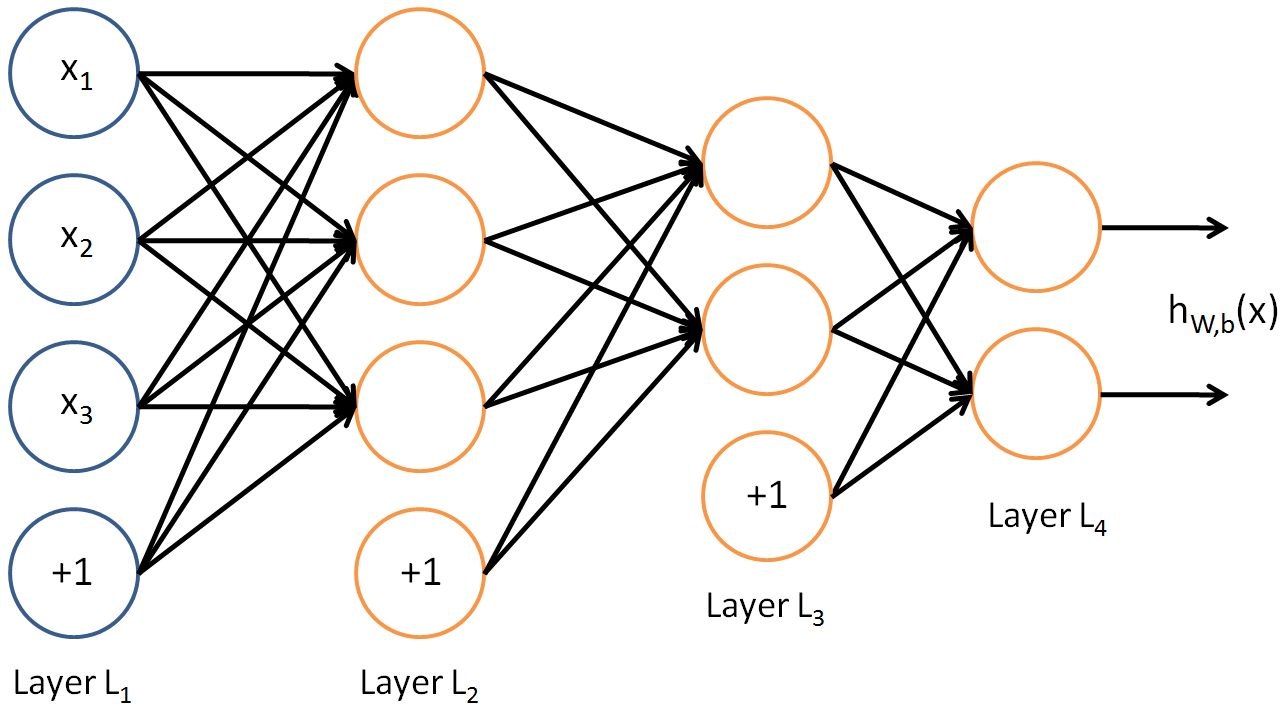
\includegraphics[width=0.45\linewidth]{UFLDL_ANN}
			\end{center}
			\caption{Illustration of a simple ANN, taken from \cite{ufldl}.}
			\label{fig:ufldl_ann}
		\end{figure}

		In CNNs the weights are instead sets of filter kernels that are convolved with the input image, hence the name.
		This reduces the amount of parameters to train because the weights are shared for all the pixels in an input.

		Between the filter neurons there are typically pooling layers inserted.
		These serve to further reduce and concentrate the data in the network.
		They work by nonlinearly sub-sampling the output image of a filter layer by eg. only sampling the pixel of highest intensity in each $2\times2$ pixel patch of the image (See Figure \ref{fig:lisa_cnn}).
		This also makes them more tolerant to small translations of the input image.
		\begin{figure}[H]
			\begin{center}
				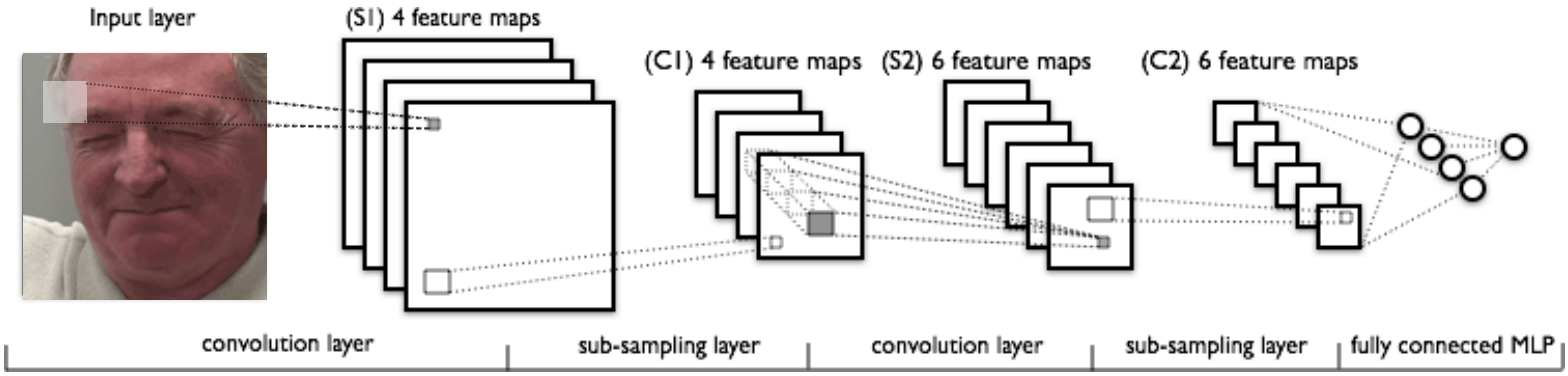
\includegraphics[width=0.8\linewidth]{CNN_example}
			\end{center}
			\caption{Illustration of a simple CNN, taken from \cite{LISAlab2015}.}
			\label{fig:lisa_cnn}
		\end{figure}
		
		The final classification is then done by either an SVM or one or more layers of traditional fully connected ANN layers like shown in Figure \ref{fig:lisa_cnn}.


		% subsection cnn_basics (end)
	
	\subsection{CNN Libraries/Toolboxes} % (fold)
		\label{sub:cnn_libraries_toolboxes}
		I have tried a couple of different libraries and toolboxes to implement the CNN:
		
		\subsubsection{DeepLearnToolbox} % (fold)
			\label{ssub:deeplearntoolbox}
			DeepLearnToolbox \cite{IMM2012-06284} is a toolbox for MATLAB, completely written in MATLAB by Rasmus Berg Palm, as part of his masters thesis at DTU.
			This toolbox offers a wide variety of functions within the domain of Deep Learning.

			This toolbox was my first attempt at implementing a CNN for pain recognition.
			I was able to install the toolbox and run test and example scripts without issue, but I never got any good results for my application.
			The problem was that with my data, processing was very slow.
			It took several hours to train a single epoch, making it next to impossible to make any progress in my development.
			I attest these problems to the fact that everything ran in MATLAB, which is known to be inefficient at times, and also partly to my inexperience with designing and training CNNs.

			% subsubsection deeplearntoolbox (end)

		\subsubsection{Deep Learning for Saliency} % (fold)
			\label{ssub:deep_learning_for_saliency}
			As described in Section \ref{sub:related_works}, a system for predicting eye fixations using CNNs has been implemented.
			I tried briefly to use thier code \cite{Shen2012a}, but found quickly that it written very much was written with their application in mind, and did not easily generalize. 

			% subsubsection deep_learning_for_saliency (end)

		\subsubsection{MatConvNet} % (fold)
			\label{ssub:matconvnet}
			MatConvNet \cite{Lenc2014} is an Open-Source MATLAB toolbox for CNNs written by \emph{vlfeat.org}, known for their excellent Computer Vision toolbox for MATLAB.
			The toolbox is implemented efficiently in C++ and in CUDA for GPU acceleration on NVIDIA hardware.\footnote{
				See Appendix \ref{sec:gpu_acceleration_of_cnn_training} for more on how to enable GPU acceleration with MatConvNet
				} 
			The code is compiled locally and have \texttt{.mex} wrappers so that it can be executed from MATLAB like any other MATLAB function.
			This is the toolbox I the majority of my time using.
		
			% subsubsection matconvnet (end)
		
		\subsubsection{Caffe} % (fold)
			\label{ssub:caffe}
			Caffe \cite{jia2014caffe} is much like MatConvNet a framework for implementing CNNs implemented in C++ and CUDA with tie-ins to MATLAB.
			Caffe seems to be the best freely available CNN framework at the moment, but an official port for Windows is not available yet, so using it was not an option for this project.

			% subsubsection caffe (end)

		% subsection cnn_libraries_toolboxes (end)

	\subsection{CNN Architecture} % (fold)
		\label{sub:cnn_architecture}
		% Selection of toolbox
		% Work from example
		% Different tests
		

		% subsection cnn_architecture (end)

	\subsection{Discussion} % (fold)
		\label{sub:cnn_discussion}
		

		% subsection discussion (end)

	% Noget om at det ikke kom til at virke
		% Hvad intensionen var
		% Hvilke værktøjer er anvendt
			% Sammenligning af værktøjer
		% Hvilke metoder er prøvet
		% Hvordan er netvæket sat op
		% Hvordan CNN overordnet virker
		% Mulige årsager til at det mislykkedes
			% For lidt data
			% For lidt tid
			% For lidt erfaring
			% Noget med autoencoder
			% Noget med opsætning af regularisereings parametere
			% Noget med hyperparametre
	
	% section convolutional_neural_network_method (end)

\end{document}